%============================================================================
% tento soubor pouzijte jako zaklad
% (c) 2008 Michal Bidlo
% E-mail: bidlom AT fit vutbr cz
%============================================================================
% kodovaní: iso-8859-2 (zmena prikazem iconv, recode nebo cstocs)
%----------------------------------------------------------------------------
% zpracování: make, make pdf, make desky, make clean
% připomínky posílejte na e-mail: bidlom AT fit.vutbr.cz
% vim: set syntax=tex encoding=latin2:
%============================================================================
\documentclass[cover]{fitthesis} % odevzdani do wisu - odkazy, na ktere se da klikat
%\documentclass[cover,print]{fitthesis} % pro tisk - na odkazy se neda klikat
%\documentclass[english,print]{fitthesis} % pro tisk - na odkazy se neda klikat
%      \documentclass[english]{fitthesis}
% * Je-li prace psana v anglickem jazyce, je zapotrebi u tridy pouzit 
%   parametr english nasledovne:
%      \documentclass[english]{fitthesis}
% * Neprejete-li si vysazet na prvni strane dokumentu desky, zruste 
%   parametr cover

% zde zvolime kodovani, ve kterem je napsan text prace
% "latin2" pro iso8859-2 nebo "cp1250" pro windows-1250, "utf8" pro "utf-8"
%\usepackage{ucs}
\usepackage[utf8]{inputenc}
\usepackage[T1, IL2]{fontenc}
\usepackage{url}
\DeclareUrlCommand\url{\def\UrlLeft{<}\def\UrlRight{>} \urlstyle{tt}}

%zde muzeme vlozit vlastni balicky


% =======================================================================
% balíček "hyperref" vytváří klikací odkazy v pdf, pokud tedy použijeme pdflatex
% problém je, že balíček hyperref musí být uveden jako poslední, takže nemůže
% být v šabloně
\ifWis
\ifx\pdfoutput\undefined % nejedeme pod pdflatexem
\else
  \usepackage{color}
  \usepackage[unicode,colorlinks,hyperindex,plainpages=false,pdftex]{hyperref}
  \definecolor{links}{rgb}{0.4,0.5,0}
  \definecolor{anchors}{rgb}{1,0,0}
  \def\AnchorColor{anchors}
  \def\LinkColor{links}
  \def\pdfBorderAttrs{/Border [0 0 0] }  % bez okrajů kolem odkazů
  \pdfcompresslevel=9
\fi
\fi

%Informace o praci/projektu
%---------------------------------------------------------------------------
\projectinfo{
  %Prace
  project=BP,            %typ prace BP/SP/DP/DR
  year=2015,             %rok
  date=\today,           %datum odevzdani
  %Nazev prace
  title.cs={Automatizovaná analýza WWW stránek},  %nazev prace v cestine
  title.en={Automated Web Page Analysis}, %nazev prace v anglictine
  %Autor
  author={Nikita Vaňků},   %jmeno prijmeni autora
  %author.title.p=Bc., %titul pred jmenem (nepovinne)
  %author.title.a=PhD, %titul za jmenem (nepovinne)
  %Ustav
  department=UPSY, % doplnte prislusnou zkratku: UPSY/UIFS/UITS/UPGM
  %Skolitel
  supervisor= Jméno Příjmení, %jmeno prijmeni skolitele
  supervisor.title.p=Ing.,   %titul pred jmenem (nepovinne)
  supervisor.title.a={Ph.D.},    %titul za jmenem (nepovinne)
  %Klicova slova, abstrakty, prohlaseni a podekovani je mozne definovat 
  %bud pomoci nasledujicich parametru nebo pomoci vyhrazenych maker (viz dale)
  %===========================================================================
  %Klicova slova
  keywords.cs={Klíčová slova v českém jazyce.}, %klicova slova v ceskem jazyce
  keywords.en={Klíčová slova v anglickém jazyce.}, %klicova slova v anglickem jazyce
  %Abstract
  abstract.cs={Výtah (abstrakt) práce v českém jazyce.}, % abstrakt v ceskem jazyce
  abstract.en={Výtah (abstrakt) práce v anglickém jazyce.}, % abstrakt v anglickem jazyce
  %Prohlaseni
  declaration={Prohlašuji, že jsem tuto bakalářskou práci vypracoval samostatně pod vedením pana ...},
  %Podekovani (nepovinne)
  acknowledgment={Zde je možné uvést poděkování vedoucímu práce a těm, kteří poskytli odbornou pomoc.} % nepovinne
}

%Abstrakt (cesky, anglicky)
\abstract[cs]{Cílem teto práce je vytvořit nástroj na automatickou analýzu webových stránek v rámci jedné domény.
Problém jsem vyřešila vytvořením webového pavouka, který mapuje a analyzuje zdroje domény.
Vytvořený pavouk ukazuje, že analýza některých domén je záležitost procházení tisíce sránek.}
%\abstract[en]{Do tohoto odstavce bude zapsán výtah (abstrakt) práce v anglickém jazyce.}

%Klicova slova (cesky, anglicky)
%\keywords[cs]{Sem budou zapsána jednotlivá klíčová slova v českém jazyce, oddělená čárkami.}
%\keywords[en]{Sem budou zapsána jednotlivá klíčová slova v anglickém jazyce, oddělená čárkami.}

%Prohlaseni
\declaration{Prohlašuji, že jsem tuto bakalářskou práci vypracovala samostatně pod vedením pana Ing. Radek Burget, Ph.D.
Další informace mi poskytli můj Team Leader František Tröster.
Uvedla jsem všechny literární prameny a publikace, ze kterých jsem čerpala.}

%Podekovani (nepovinne)
%\acknowledgment{V této sekci je možno uvést poděkování vedoucímu práce a těm, kteří poskytli odbornou pomoc
%(externí zadavatel, konzultant, apod.).}

\begin{document}
  % Vysazeni titulnich stran
  % ----------------------------------------------
  \maketitle
  % Obsah
  % ----------------------------------------------
  \tableofcontents
  
  % Seznam obrazku a tabulek (pokud prace obsahuje velke mnozstvi obrazku, tak se to hodi)
  % \listoffigures
  % \listoftables 

  % Text prace
  % ----------------------------------------------
  %=========================================================================

\chapter{�vod}
World Wide Web (d�le jen WWW) dokumenty jsou st�le v�ce vyu��van�j��mi sd�lovac�mi prost�edky. Jejich po�et neust�le roste [zdroj]. Vyu�it� WWW dokument� se nach�z�. WWW dokumenty se vyu��vaj� pro �irokou �k�lu ��el�. M��eme narazit na dokumenty se sp��e statick�m obsahem jako jsou blogy, firemn� reprezentace atd. M��eme ale tak� narazit na dokumenty s~kompletn� dynamicky generovan�m obsahem jako jsou nap�. internetov� vyhled�va�e. informa�n� syst�my, webov� aplikace aj.

Mno�stv� webov�ch str�nek na dom�n� je t�m�� neomezen�. Na internetu lze naj�t dom�ny o~n�kolika str�nek, ale i dom�ny jejich� obsah roste po v�ce jak deset let a obsahuj� stovky a� tis�ce. Takov� dom�ny pak cyklicky proch�zej� refactoringem k�du �i cel�ho syst�mu. M��e se pak st�t, �e se �ada str�nek zapomene �i vytrat�. �i naopak, �e syst�m roste a nalepuj� se na n�j dal�� a dal�� ��sti, mnohdy zbyte�n�. Stejn� tak se star� neodstran�, t�eba i z~d�vodu, �e v~program�torsk�m t�mu "nikdo nem� tu�en� co to d�l� a co se stane, pokud se to d� pry�". 

Z~tohoto a dal��ch d�vod� vyu��vaj� t�my mnoho n�stroj�, kter� analyzuj� zpracov�n� po�adavku serveru. Jedn� se o~m��en� rychlosti zpracov�n� backendu a frontendu. Velikost stahovan�ch klientsk�ch zdroj� jako jsou nap��klad soubory kask�dov�ch styl�, obr�zky �i Javascriptov� knihovny. Jednim z~t�chto n�stroj� jsou Webov� crawlery, neboli pavouci. 

Pavouci na�li nejv�t�� vyu�it� hlavn� u~internetov�ch vyhledava��. Jsou navr�eni tak taby v~kr�tk�m �ase dok�zali zpracov�vat najednou velk� mno�stv� str�nek z~r�zn�ch dom�n. P�i zpracov�v�n� hled� odkazy na dal�� str�nky a ty tak� analyzuje. Vzhledem k~velikosti a ne�stal�ho r�sta pavouci mnohdy svou pr�ci nikdy nekon��, nebo jsou spou�t�ni pravideln�. �loha pavouk� m��e b�t r�zn�. 

M�m c�lem je vytvo�it pavouka, kter� bude analyzovat pouze jednu dom�nu. P�edpokl�d� se, tedy �e bude zpracov�vat pouh� stovky a� tis�ce str�nek. V�stupem anal�zy maj� b�t program�tor�m u�ite�n� data jako grafick� zobrazen� prov�zanosti str�nek. M��en� rychlosti a anal�za stahov�n� str�nek. Rendering str�nek. Sou��st� anal�zy je mo�no tak� sledov�n� chyb Javascriptu �i validace DOM objektu. 

V~t�to pr�ci se budu v�novat n�kolika hlavn�ch ��st� t�to problematiky. Prvn� ��st bude v�nov�na anal�ze problematiky pavouk�. V~druh� ��sti zpracuji n�vrh vlastn�ho pavouka. Ve t�et� ��sti budu �e�it implementaci vyhotoven�ho n�vrhu a posledn� ��st je v�nov�na experiment�m s~pavoukem a v�sledky jeho anal�z.

\newpage
\chapter{Teorie}
Tato kapitola je v�nov�na teoritick�m zpracov�n�m problematiky anal�zy webov�ch str�nek. Web lze reprezentovat jako graf, ve kter�m uzly jsou dokumenty identifikovan� URL a hrany hypertextov� odkazy. C�lem pavouka je proj�t podgraf tohoto grafu vymezen� po��ta�n�m uzlem a dal��mi omezen�ny jako specifikace povolen�ch dom�n. Robot p�i proch�zen� m��e prov�st jednoduchou anal�zu dokumentu jako zaznamen�n� n�vratov�ho kodu serveru, extrakce hypertextov�ch odkaz�, vyhled�n� formul��� apod.

\section{Sou�asn� pavouci}
\label{sec:today_crawlers}
Dnes se pavouci vyu��vaj� p�ev�n� k~indexov�n� internetu pro internetov� vyhled�va�e. Mezi ty nejv�ce zn�me m��eme za�adit Google �i Bing. Detaily implementace t�chto pavouk� jsou pochopiteln� utajeny. Krom� pavouk� analyzuj�c� cel� internet bez omezen� existuje i cel� �ada �zce specializovan�ch pavouk� pro ur�itou �innost. Nap��klad \texttt{skipfish\footnote{https://code.google.com/p/skipfish/}} je Open Source pavouk testuj�c� zabezpe�en� dom�ny a odhaluje slab� m�sta, kter� by mohli vyu��t �to�n�ci. \texttt{HTTrack\footnote{https://www.httrack.com/}} je pavouk, kter� po zad�n� adresy proch�z� ve�ker� jej� obsah a stahuje ho do ulo�i�t�. Str�nky lze potom prohl��et Offline.

Pavouci ve sv� povaze p�istupuj� k~webov�m server�m v~ohromn� v�t��m m���tk�m ne� oby�ejn� u�ivatel. Toto m��e znamenat, �e server klasifikuje pavouk jako nebezpe�n�ho robota �i snad pokus o~DDos �tok a zak�e pavouk�v p��stup k~dat�m serveru. Tento p��pad m��e nastat i v~na�� aplikaci. Bohu�el ka�d� webov� server m��e nastavit tento limit na jin� �rovni a ka�d� se tak� v~p��pad� p�ekro�en� limitu m��e zachovat jinak. N�kter� servery se mohou br�nit sn��en�m priority odpov�d�, jin� neodpov�d�n�m �pln�.

\section{Anal�za URL}
\label{sec:analysis}
Uniform Resource Locator (d�le jen URL, neboli t� adresa) jsou definov�ny v~\texttt{RFC 3986}\cite{rfc3986}. Je pot�eba rozli�it relativn� a absolutn� adresu. V~p��pad� relativn� adresy se zohled�uje aktualn� adresa dokumentu. Sou��st� URL m��e b�t t� kotva, kotva je definov�na atributem \texttt{id} v~elementu \texttt{<a>}, kotvy nemaj� pro pavouka ��dn� v�znam a jsou tedy ignorov�ny. V~p��pad� nalezen� v�t��ho mno�stv� odkaz� se stejnou adresou v~dokumentu, pavouk se zachov� jako by pracoval s~adresou jedinou.

Pavouk by tak� m�l b�t p�ipraven �elit generovan�m hypertexov�m odkaz�m, jako jsou str�nky s~dynamick�m obsahem, kter� se mohou jevit z~pohledu pavouka jako nekone�n�.\cite{mining}

Velk�m o���kem mohou b�t t� \texttt{GET} parametry, kter� jsou sou��st� URL. Tyto parametry maj� nejednozna�n� v�znam a pavouk nem��e v�d�t, zda-li jim m� v�novat pozornost. GET parametr m��e i nemus� m�t ��dnou v�hu na vykreslen� dokumentu. 
Mohou existovat i str�nky obsahuj�c� odkazy s~velk�m mno�stv�m opakuj�c�ch se GET parametr�. Pavouk by m�l b�t schopen tyto odkazy normalizovat a t�m nevid�t rozd�l mezi odkazem

\begin{center}
  \url{http://www.domain.com/index.php?param1=1&param2=2}\\
  a odkazem\\
  \url{htpp://www.domain.com/index.php?param2=2&param1=1}
\end{center}
\section{Extrakce URL}
\label{sec:extraction}
Extrakce adres je mo�n� anal�zou HTML webov�ch dokument�. Prozkoum�n�m vybran�ch element�, m��eme z�skat pot�ebn� odkazy. Mezi zmi�ovan� elementy pat��\footnote{Je pot�eba br�t v~potaz, �e URL  mohou b�t v~dokumentu vlo�eny tak� jako pouh� text �i p�i zpracov�n� ud�losti javascriptem. Tyto odkazy pavouk pochopiteln� nenajde.}.

\begin{itemize}
	\item \texttt{<a></a>} atribut \texttt{href}
	\item \texttt{<form></form>} atribut \texttt{action}
	\item \texttt{<link>} atribut \texttt{href}
	\item \texttt{<script></script>} atribut \texttt{src}
	\item \texttt{<style></style>} atribut \texttt{src}
\end{itemize}

V~z�vislosti na povaze atributu je mo�no p�edpov�dat na jak� mime typ webov�ho objektu odkaz ukazuje. Jestli�e extrahujeme atributy src z~tagu \texttt{script} a \texttt{style}, m��eme si b�t jisti �e mime type bude text/css �i text/javascript. Takto m��eme konkr�tizovat zpracov�n� odkaz�, jeliko� odkazy v~t�chto souborech hledat nebude.e

\section{Zaznamen�n� �asov�ch ud�lost�}
\label{sec:time_events}
Pro u�ivatele je d�le�it� co nejkrat�� �as mezi odesl�n�m po�adavku na server a zobrazen� str�nky. Tento �as je mo�n� rozd�lit na dv� hlavn� ��sti a to:
\begin{itemize}
 \item �as str�veny zpracov�n�m po�adavku na serveru - \texttt{Backend}
 \item �as str�ven� sta�en� a zobrazen� zdrojov�ch dokument� - \texttt{Frontend}
\end{itemize}
Webov� str�nka, kter� se zobraz� u�ivateli v~prohl��e�i je mnohdy slo�ena z~v�ce soubor�. Jedn� se jednak o~HTML/XML dokument, ale tak� o~obr�zky, Kask�dove styly, Javascript a dal�� soubory. Modern� prohl��e�e dnes dok�� stahovat v�ce soubor� z~jednoho serveru najednou aby �as str�ven� stahov�n�m co nejv�ce urychlily. Mno�stv� vl�ken se v�ak u~ka�d�ho prohl��e�e li�� a u�ivatel m��e s~touto hodnotou manipulovat. (zdroj)

Nam��en� �asy mus�me tak� pova�ovat za nep��li� pr�kazn�. Server m��e odpov�dat rychleji �i pomaleji v~z�vislosti na sou�asn�m zat��en� u�ivatelsk�mi po�adavky. Pr�kazn� m��en� by se dalo dos�hnout pomoc� pravideln�ho a dlouhodob�ho m��en�

\newpage
\chapter{N�vrh aplikace}
\label{ch:plan}
Aplikace je slo�ena z~n�kolika ��st�. Jedn� se o~algoritmus pavouka, kter� stahuje a analyzuje dokumenty. Datab�zov�m ulo�i�t�m, kter� uchov�v� analyzovan� data a grafick� nadstavba (GUI) p�es kterou je aplikace ��zena. Pro vykreslov�n� dokument� jsou vyu�ity technologie Headless Browseru, v~tomto p��pad� byl vyu�it PhantomJS, kter� pracuje na vykreslovac�m j�d�e WebKit.

\section{Java}
\label{sec:java}
Byla vyu�ita platforma Java s~platformou JavaFX, kter� umo��uje tvorbu Rich Internet Applications\cite{java}. JavaFX aplikace je mo�no vyu��t i jako desktopov� aplikace. Aplikace vytvo�ena sou��st� t�to pr�ce byla naprogramov�na pro Java 8, JavaFX 8.

\section{Modifikace prohled�van�ho prostoru}
C�lem aplikaci je analyzovat pouze jedinou dom�nu. P�i prohled�v�n� je tedy nutno zamezit zabloud�n� pavouka na ciz� dom�ny a prohled�v�n� zcela jin� ��sti internetu. Toto je dosa�eno kontrolou dom�ny nejvy���ho soukrom�ho ��du spole�n� s~ve�ejn�m suffixem. Pokud se dom�na tohoto ��du nebo suffix li��, adresa se neprohled�v�.

Je t�eba tak� po��tat s~t�m, �e mno�stv� dokument� a odkaz� na dom�n� nen� p�edem zn�mo. Dom�na m��e obsahovat n�kolik des�tek dokument�, ale i n�kolik stovek. Aplikace mus� b�t na tuto skute�nost p�ipravena a v~p��pad� proch�zen� takto velk� dom�ny zareagovat. Toto je uskute�n�no stanoven�m maxim�ln� hloubky prohled�v�n�. P�ed prohled�n�m prvn�ho dokumentu je aktualn� hloubka 0 a ka�d�m dal��m dokumentem se hodnota zv��� o~1. V~p��pad� dosa�en� maxim�ln� hloubky prohled�v�n� se z~tohoto dokumentu neextraktuj� dal�� adresy.

Mno�stv� webov�ch str�nek obsahuje mnohdy ��st s~dynamicky generovan�m obsahem, jeho� anal�za by spot�ebovala p��li� velk� mno�stv� prost�edk�, �i n�s tato ��st nezaj�m�. M��e se jednat o~blogy, fora, �i jin� aplikace kde obsah tvo�� p�ev�n� u�ivatel� str�nek. V~opa�n�m p��pad� mohou b�t webov� str�nky p��tomny na n�kolika dom�n najednou. Z~tohoto d�vodu se prohled�v�n� ��d� taky podle u�ivatelem definovan�ch pravidel. Pravidlo, kter� zamez� prohled�v�n� ��sti dom�ny (subdom�ny) a omez� tak prohled�van� prostor a pravidlo, kter� naopak povol� prohled�v�n� na dal��ch dom�n�ch a zv�t�� t�m prohled�van� prostor.

\section{Anal�za DOM objektu}
\label{sec:dom_analysis}
Extrakce adres z~HTML dokument� je mo�n� za pomoc� prohled�n� Document Object Modelu (d�le jen DOM). V~objektu se hledaj� elementy a atributy zm�n�n� v~\ref{sec:extraction}. Vyta�en� adresy se mus� d�le zpracovat jak bylo pops�no v~\ref{sec:analysis}, k~adrese se tak� p��d� z�znam na kter�m dokumentu byl nalezen a n�sledn� se vlo�� do fronty ke zpracov�n�.

Pro pr�ci s~DOM objektem a extrakci adres je vyu�it HTML parser \texttt{jsoup}. Jedna z~vlastnost� tohoto parseru je um�t se vypo��dat s~nevalidn�m dokumentem. Chybn�m pou�it�m tagu apod. \cite{jsoup}

\section{Ulo�en� dat}
\label{sec:data_storage}
Jednou z~hlavn�ch ot�zek bylo kam ulo�it data vytvo�en� anal�zou. P�i p��prav� aplikace jsem tuto ot�zku hluboce podcenila, prvn� zku�ebn� prototypy ukl�daly v�echny data do RAM pam�ti. I~u~velice mal�ch webov�ch str�nek se vytvo�ilo velk� mno�stv� objekt�. Takov� velk� mno�stv� neust�le ulo�en�ch objekt� zp�sobilo naalokov�n� n�kolik GiB pam�ti a n�sledn�ho p�du aplikace.

Rozhodla jsem se vyu��t datab�zi pro ukl�d�n� v�t�inu dat.

\subsection{Datab�ze}
\label{subsec:data_database}
Jako datab�ze byla zvolena \texttt{OrientDB 2.0.X Community Eddition\footnote{V pr�b�hu v�voje aplikace byla verze n�kolikr�t aktualizovan�}}, jedn� se o~hybridn� NoSQL datab�ze umo��uj�ci pracovat jak v~Dokument (\texttt{MongoDB}) tak Grafov�m (\texttt{Neo4j}) modu.

Aby aplikace nemusela skladovat v~pam�ti p��li� velk� mno�stv� dat, data se co nejd��ve po zpracov�n� p�esunou do datab�ze. Jeliko� zpracovan� data ve sv� podstat� vytv��� orientovan� graf webov�ch dokument�, byla pro tuto pot�ebu zvolena grafov� datab�ze. Zp�sob ulo�en� dat v~datab�zi tedy co nejv�ce p�ipom�n� zp�sobu ulo�en� dat na dom�n�. 

Grafov� datab�ze je sestavena stejn� jako graf ze dvou z�kladn�ch stavebn�ch prvk�. Vrcholy a hrany mezi vrcholy. Jako vrcholy si m��eme nap��klad p�edstavi dokumenty. Hrany by pot� mohly b�t odkazy mezi t�mito dokumenty. V~sekci Implementace datab�ze \ref{sec:impl_database} je v�novan� ��st n�vrhu datab�ze a jej� propojen� s~aplikac�.

\subsection{Souborov� syst�m}
\label{subsec:data_filesystem}
Pokud se s~ka�d�m webov�m objektem do datab�ze ulo�� i identifik�tor, je pak mo�no tento identifik�tor vyu��t k~sestaven� struktury adres��� na souborov�m syst�mu. Do t�chto adres��� by se ukl�dala data, kter� by jednodu�e nebylo praktick� ukl�dat do datab�ze. Jedn� se o~vykreslen� webov� sn�mky a dal�� p��li� velk� data.

Je nutno tak� podotknout, �e takto ulo�en� data na v�ce m�st� ztr�c� integritu. Datab�ze m��e b�t p��tomn� na vzd�len�m serveru a sta�� n�m zn�t pouze adresu a p��stupov� �daje ke zp��stupn�n� jejich dat. V~p��pad� souborov�ho syst�mu mus� b�t tento syst�m v�dy n�jak�m zp�sobem p�ipojen k~syst�mu na kter�m b�� aplikace.

\section{Vykreslen� dokumentu}
\label{sec:resource rendering}
Pro vykreslov�n� webov�ch dokumentu byl vyu�it Headless browser \texttt{PhantomJS 2.0}. PhantomJS obsahuje vykreslovac� j�dro WebKit, lze s~n�m tedy emulovat vykreslov�n� podobn� prohl��e��m se stejn�m j�drem jako je nap� Google Chrome, Safari �i Opera \cite{phantomjs}. 

PhantomJS je pln� ovladateln� Javascriptem. Program se spust� s~parametrem cesty k~javascriptov�mu souboru, kter� obsahuje ovl�dac� skript prohl��e�e. Prohl��e� vykon� instrukce v~tomto skriptu a pot� se ukon��. Aplikace spou�t� prohl��e� s~jednoduch�m skriptem, kter� p�istoup� na adresu, obsah vykresl� do souboru a pot� se ukon��.

\section{Projekty}
\label{sec:projects}
Aplikace by m�la b�t znovupou�iteln� pro v�t�� po�et anal�z dom�n a jejich proch�zen�. Proto jsem se rozhodla anal�zy rozd�lit na tzv. projekty. Jeden projekt je anal�za jedn� dom�ny. Projekt je mo�n� vytvo�it, spustit anal�zu, prohl��et v�sledky a smazat.

Projekt je prim�rn� ulo�en v~datab�zi s~v�t�inou dat. Data, nep��li� vhodn� ulo�it do datab�ze jsou ulo�ena v~souborov�m syst�mu, projekt by m�l b�t schopen je nal�zt.

\section{N�vrh u�ivatelsk�ho rozhran�}
\label{sec:draft_gui}
P�i n�vrhu jsem se pokusila kl�st d�raz na jednoduch� ovl�d�n� aby program byl schopen ovl�dat i mirn� pokro�il� u�ivatel internetu. 

U�ivatel by m�l b�t schopen v~aplikaci pln� pracovat s~projekty. Tedy m�l by m�t mo�nost vytvo�it nov� projekt, nebo otev��t ji� vytvo�en�. Spustit anal�zu dom�ny �i smazat ji� hotovou anal�zu a hlavn� proch�zet v�sledky anal�zy. Toto se uk�zalo jako nejslo�it�j�� probl�m, jeliko� u�ivatel by m�l intuitivn� proch�zet grafem.
Zvolila jsem zp�sob zobrazen� pr�v� proch�zen�ho uzlu a jeho nejbli��� okol� v~orientovan�m grafu. Po poklik�n� na kter�koliv vrchol v~zobrazen� se tento vrchol a jeho nejbli��� okol� otev�e.

\newpage
\chapter{Implementace aplikace}
\label{ch:implementation}
Tato kapitola je v�nov�na implementace n�vrhu v~p�edchoz� kapitole a jak se z�vere�n� implementace oproti n�vrhu zm�nila.

Aplikace JavaFX podl�haj� MVC n�vrhu tedy \texttt{Model-View-Controller}. J�dro aplikace, tedy datov� model je odd�len od zobrazovac� vrstvy. S~datov�m modelem p��mo komunikuje Controller, tedy ��d�c� prvek. ��d�c� prvek komunikuje takt� s~View, tedy pohledem, p�es mno�inu komponent, kter� je v~pohledu definovan�. ��d�c� prvek sleduje reaguje na zpr�vy zaslan� pohledem, kter� zpracov�v� a p�epos�l� d�le. Pokud se jedn� o~vlastnosti �i parametry modelu, ��d�c� prvek je m��e pevn� obou �i jednostran� sv�zat s~komponentou. Nap�. vlastnost modelu datov�ho typu String m��e b�t sv�z�n� s~komponentou text v~pohledu. P�i jak�koliv zm�ny t�to vlastnosti v~modelu, je komponenta aktualizov�na.

V~datov�m modelu je obsa�ena hlavn� funkcionalita aplikace. J�dro cel� aplikace zastupuje t��da \texttt{Crawler}. Crawler je spu�t�n ve stejn�m vl�kn� jako ��d�c� prvky a pohledy. Funguje jako hlavn� ��d�c� jednotka. Pokud u�ivatel zad� p��kaz k~modifikaci projektu �i spu�t�n� anal�zy Crawler p�epo�le p��kaz slu�b�m v~samostatn�ch vl�knech, nebo vytvo�� dedikovan� vl�kno pro spln�n� �lohy. Toto se prov�d� zejm�na p�i zpracov�v�n� slo�it�ch p��kaz�, kter� by �inily u�ivatelsk� rozhran� neresponzivn�.

Mezi slu�by, kter� spravuje t��da crawler pat�� sb�ra� odkaz� (sestaven� grafu) a post anal�za (vykreslov�n� str�nek obsahuj�c� DOM objekt).

\section{Anal�za dom�ny}
\label{sec:domain_analysis}

Slu�by, kter� zprost�edkov�vaj� anal�zu dom�ny s~hlavn� t��dou komunikuj� pouze omezenou mno�inou zpr�v oznamuj�c� �sp�ch �i ne�sp�ch anal�zy. Zpracovan� data jsou p�ed�na prost�ednictv�m datab�ze �i souborov�ho syst�mu.

\subsection{Prvn� ��st - tvorba grafu}
\label{subsec:domain_analysis_graph}

Slu�ba, sestavuj�c� graf webov�ch objektu pracuje jako fronta odkazu. Z~fronty slu�ba odebere odkaz, u~kter�ho nejd��ve zjist�, zda-li se odkaz nach�z� v~prohled�van�m prostoru. Pokud je objekt mimo prohledan� prostor do datab�ze se ulo�� objekt s~minim�ln�m mno�stv�m informac�. V~opa�n�m p��pad� je objekt sta�en a prozkoum�m n�strojem \texttt{jsoup}. N�strojem jsou prozkoum�ny tagy a jejich atributy zm�n�ne v~sekci \ref{sec:extraction}, ve�ker� nalezen� odkazy jsou vlo�eny do zp�t do fronty. Jestli-�e se jedn� o~objekt bez DOM ��sti je objekt pova�ov�n za soubor a do datab�ze vlo�en jeho z�znam. Po ulo�en� objektu je do datab�ze vlo�en tak� odkaz samotn� v~podob� hrany. Slu�ba si tak� udr�uje v~pam�ti objekty, kter� ji� jednou zpracovala. Nedoch�z� tak k~opakovan�mu stahov�n� a zpracov�n� ji� hotov�ch objekt�.

\begin{figure}[H]
  \centering
  \scriptsize
  \includesvg[width=13cm]{miner}
  \caption{Proces zpracov�n� odkazu} \label{fig:miner}
\end{figure}


\subsection{Druh� ��st - (post processing)}
\label{subsec.domain_analysis_postprocessing}

V~�ase spu�t�n� druh� ��sti anal�zy je v~datab�zi p��tomen ji� hotov� graf objektu s~jejich z�kladn�mi informacemi. Slu�ba z~datab�ze extrahuje objekty, kter� obsahuj� DOM (��st) a pro ka�d� z~t�chto objekt� nejd��ve vytvo�� sv� m�sto ve stromu souborov�ho syst�mu, kam bude slu�ba pozd�ji ukl�dat informace o~objektu. Cesta k~tomuto adres��i se skl�d� z~n�zvu projektu a specialn�ho identif�ktoru p�i�azen�ho Orient datab�z�. Po dokon�en� p��pravy zapo�ne spou�t�n� extern�ho webov�ho prohl��e�e \texttt{PhantomJS} se skriptem, kter� webovou str�nku vykresl� do obr�zku a z�rove� zaznamen� Javascriptov� konzolov� v�stup p�i zpracov�n� str�nky do soubory. V~konzolov�m v�stupu se �asto objevuj� chyby p�i vykreslov�n� str�nek.


\section{Datab�ze}
\label{sec:impl_database}

Orient Datab�ze m��e pracovat s~objekty ve dvou modifikac�ch. Jako dokumenty a jako graf. Ka�d� z~t�chto dvou modu se hod� pro jinou aplikaci. Jak ji� bylo zm�n�no v~sekci \ref{subsec:data_database}, pro ukl�d�n� webov�ch objektu je p�irozen�j�� pou��t mod grafu. Naopak pro pr�ci s~frontou zm�n�nou v~sekci \ref{subsec:domain_analysis_graph} je v�hodn�j�� pracovat s~dokumenty. 
Aplikace je propojena s~datab�z� p�es nativn� Java konektor. Konektor je schopen pracovat v~t�chto dvou modech. Nab�z� pro to �adu konstrukc� a metod. Orient datab�ze umo��uje taky pou��t SQL jazyk, tento jazyk je narozd�l od nap�. Oracle SQL jazyku zna�n� omezen�, ale obsahuje �adu z�kladn�ch agrega�n�ch metod a klauzul�, kter� jsou pro aplikaci dosta�uj�c�.

Orient Datab�ze nezn� pojem tabulka, m�sto n� zav�d� pojem t��da. T��da maj� schopnost d�di�nosti. Pokud chce u�ivatel vytvo�it t��du, kter� bude uzlem nebo hranou v~grafu, vytvo�� kter� bude d�dit vlastnosti abstraktn�ch t��d V~�i E. Tyto t��dy jsou ji� v~datab�zi p��tomny po jej�m vytvo�en�. V~p��pad�, �e u�ivatel vytvo�� t��du, kter� nebude d�dit vlastnosti z~jedn� z~t�chto t��d, bude tato t��da ch�pana jako dokument.

Orient Datab�ze ukl�d� z�znamy t��d do tzv. clusteru. Ka�d� t��da m� alespo� jeden cluster do kter�ho ukl�d� sv� data. Clustery jsou od sebe fyzicky odd�leny. Clusteru m��e b�t v�ce, vkl�d�n� do nich m��e b�t prov�d�no p��mo �i na z�klad� algoritmu. Clustery jsou od sebe fyzicky odd�leny, tato vlastnost se vyu��v� obzvlṻ pokud datab�ze b�� v~redistribu�n�m modu na n�kolika serverov�ch jednotk�ch \cite{orient}. Spoustu datab�zi trp� p�i neust�le rostouc�m objemu dat, slo�it� dotazy v~takov�m p��pad� trvaj� mnohem d�le ne� by trvaly v~mal�ch datab�z�ch. P�itom postupem �asu se v~datab�zi za�nou objevovat data, ke kter�m se bude p�istupovat m�n� �i t�m�� vb�ec. Pokud se takov� data p�esunou do jin�ch cluster� a datab�ze pracuje s~jednim clusterem, kter� m� omezen� mno�stv� dat, lze takto rychlost dostaz� podstatn� nav��it.

\begin{figure}[H]
  \centering
  \tiny
  \includesvg[width=5cm]{clusters}
  \caption{Datab�zov� cluster}
\end{figure}

Data, kter� aplikace ukl�d� do datab�ze jsou v~podstat� rozd�len� do projekt� jak ji� bylo zm�n�no v~sekci \ref{sec:projects}. Pokud ka�d� projekt bude m�t sv� clustery, kter� se vytvo�� v�em t��d�m se kter�mi projekt pracuje lze tak spolehliv� odd�lit data ka�d� projektu a vy�e�it tak probl�m, kter� by zp�soboval rostouc� dobu vykon�van� dotaz� s~v�t��m mno�stv�m ji� analyzovan�ch projekt�.

\subsection{Schema datab�ze}

V~tabulce \ref{tab:db_classes} a diagramu \ref{fig:db_schema} je zn�zor�eno jak vypad� fin�ln� schema datab�ze. Projektov� clustery se tvo�� v~t��d�ch \texttt{Resource, Form, BlackWhitelist, LinkTo, Includes, LinkQue}. N�zev t�chto clusteru se sest�v� spojen�m n�zvu t��dy a unik�tn�mu identifik�tor�, kter� je ulo�en jako vlastnost \texttt{cluster} ve t��d� \texttt{Project}.

\begin{table}[H]
  \begin{center}
    \begin{tabular}{| c | c | l |}
      \hline
      \textbf{N�zev} & \textbf{Typ} & \textbf{Popis} \\
      \hline
      \texttt{Resource} & Vrchol & Webov� objekt \\
      \hline
      \texttt{Form} & Vrchol & Formul�� \\
      \hline
      \texttt{Project} & Vrchol & Projekt \\
      \hline
      \texttt{LinkTo} & Hrana & Odkaz mezi dokumenty \\
      \hline
      \texttt{Includes} & Hrana & P�ipojen� formul��e k~dokumentu \\
      \hline
      \texttt{Root} & Hrana & Odkaz na ko�enov� dokument prohled�van� dom�ny \\
      \hline
      \texttt{BlackWhitelist} & Vrchol & Omezen� prohled�van�ho prostoru \\
      \hline
      \texttt{LinkQue} & Dokument & Fronta pro skladov�n� odkaz� �ekaj�c� na zpracov�n� \\
      \hline
      \texttt{LinkSet} & Dokument & Mapa nav�t�ven�ch objekt� \\
      \hline
    \end{tabular}
  \end{center}
  \caption{T��dy datab�ze} \label{tab:db_classes}
\end{table}

\begin{figure}[H]
  \centering
  \tiny
  \includesvg[width=14cm]{db-schema}
  \caption{Diagram datab�ze} \label{fig:db_schema}
\end{figure}

\section{Grafick� rozhran�}
\label{sec:gui}
JavaFX umo��uje mo�nost navrhnout design ve specialn� XML konstrukci, kter� se jmenuje FXML. Designov� komponenty se zapisuj� stejn� jako XML uzly. Uzly maj� p�i�azen� indetifik�tory, kter� jsou p�ed�v�ny controlleru, tedy ovlada�i, co� mezivrstva mezi modelovac� a zobrazovac� vrstvou.

V~n�vrhu jsem grafick�mu rozhran� nev�novala p��li� mnoho �asu, fin�ln� n�vrh aplikace vznikla mno�stv�m iterac� a experiment� s~neust�lou obm�nou designov�ch komponent. Aplikace je rozd�lena do n�kolika z�lo�ek. Krom� z�lo�ek u�ivatel ovl�d� aplikaci p�es menu panel v~horn� ��sti aplikace. Ve spoedn� ��sti aplikace se nach�z� n�kolik z�lo�ek s~v�pisy konzole programu a slu�eb. Tyto v�pisy slou�� k~informov�n� u�ivatele o~�innosti aplikace, jeliko� aplikace prov�d� velk� mno�stv� operac� na pozad� a u�ivateli by se mohla zd�t jako neresponzivn�. Prav�m tla��tkem s~ikonou gumy u�ivatel sma�e obsah pr�v� zvolen�ho v�pisu.

�vodn� okno obsahuje tabulku s~projekty. Projekt je mo�no otev��t, smazat �i vytvo�it nov�.

\begin{figure}[H]
  \centering
  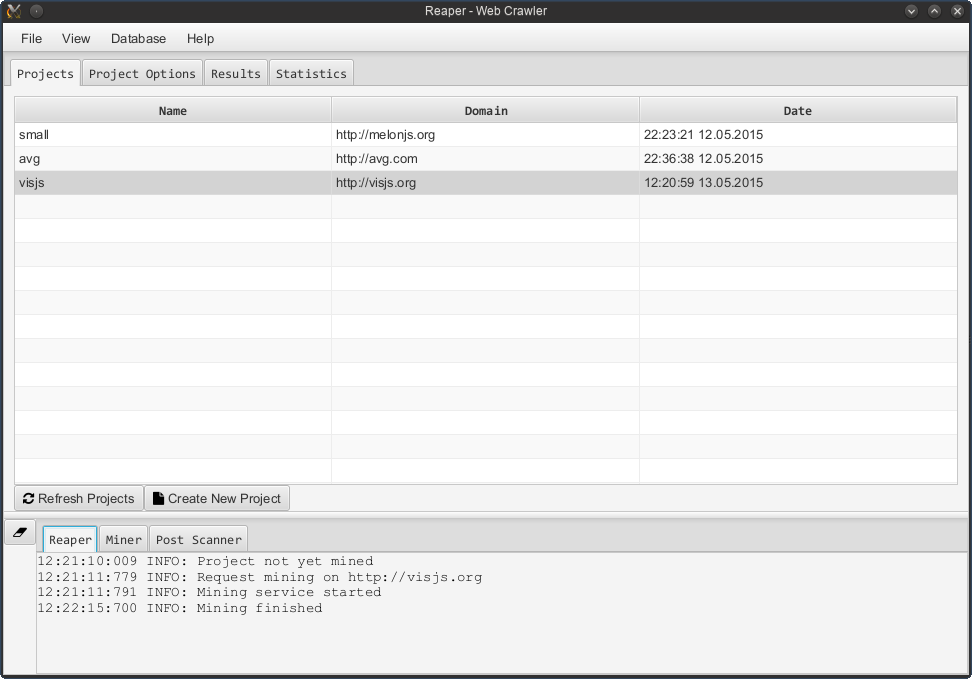
\includegraphics[scale=0.6]{reaper-projects}
  \caption{�vodn� okno} \label{fig:reaper_projects}
\end{figure}

V~t�to z�lo�ce je u�ivatel schopen zm�nit nastaven� prohled�v�n� a to konkr�tn� c�lovou dom�nu, hloubku, vymezen� prohled�van�ho prostoru. Tak� je schopen smazat data z~ji� existuj�c� anal�zy, anebo zah�jit anal�zu novou. Jak ji� bylo uvedeno v~kapitole (doplnit), anal�za prob�h� ve dvou f�z�ch. Z~d�vodu �asov� n�ro�nosti je nutn� spustit ob� f�ze manu�ln�. Jeliko� druh� f�ze zvy�uje line�rn� n�rok na prost�edky a �as k~jej� vyhotoven� a informace z�skane v~teto f�zi nemus� b�t pro u�ivatele d�le�it�.

Po spu�t�n� anal�zy aplikace uzamkne velk� mno�stv� ovl�dac�ch prvk� dokud anal�za nen� dokon�ena. Bez tohoto zabezpe�ovac�ho mechanismu by u�ivatel byl schopen vydat p��kaz k~nap��klad smaz�n� dat zat�mco jsou stahov�na a zap���inil tak nedefinovan�mu chov�n� aplikace.

\begin{figure}[H]
  \centering
  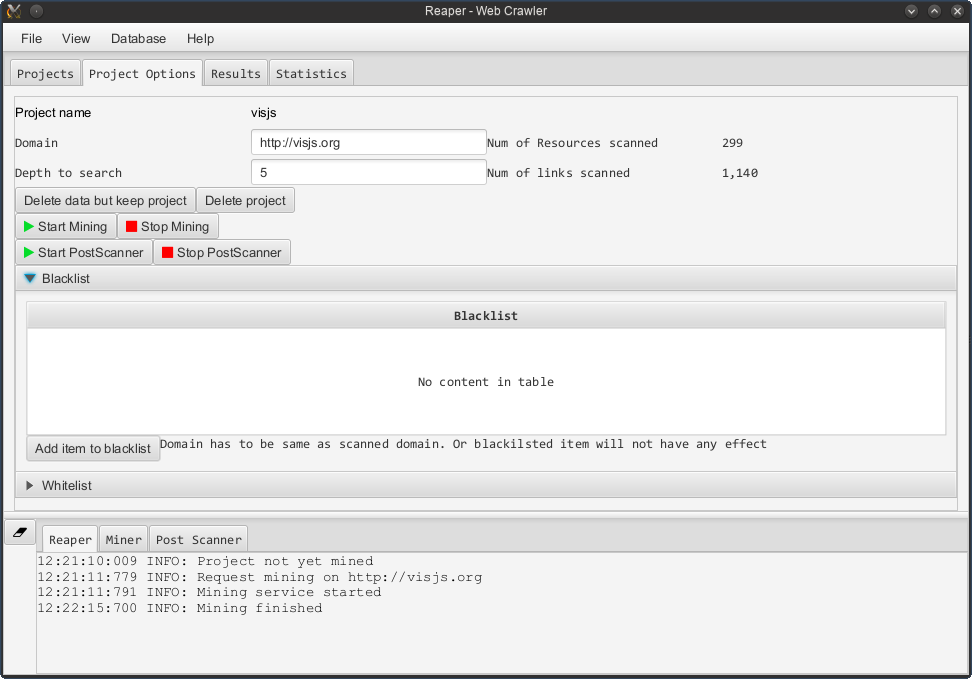
\includegraphics[scale=0.6]{reaper-projectoptions}
  \caption{Ovl�d�n� anal�zy} \label{fig:reaper_analysis}
\end{figure}


P�i na�ten� projektu se v~z�lo�ce v�sledky na�te ko�enov� objekt anal�zy. Proch�zen� v�sledk� je rozd�leno do zobrazen� grafu vlevo a seznam pr�v� zobrazen�ch objekt� v�etn� detailu proch�zen�ho objektu. 
Graf vsazen do prohl��e�e, kde jej vykresluje Javascriptov� knihovna \texttt{Vis.js} . Tato knihovna nab�z� jednoduchou funkcionalitu pro vykreslov�n� �asov�ch diagram� a graf�. Graf je vykreslen n�kolika barevn�, ka�d� z~barev ozna�uje typ webov�ho objektu. U~hran mezi uzly je taky zobrazeno ��slo, toto ��slo reprezentuje kolik odkaz� dohromady vede mezi dv�ma webov�mi objekty. V~prav�m horn�m rohu jsou p��tomny 3 checkboxy, pomoci kter�ch u�ivatel ovl�d�, jak� typy webov�ch objekt� se v~grafu zobraz�.
V~prav�m panelu je ve dvou z�lo�k�ch um�st�n seznam zobrazen�ch objekt� v~tabulce a takt� detail pr�v� proch�zen�ho objektu. Mno�stv� informac� zobran�ho v~detailu z�vis� na typu webov�ho objektu. Nap�. u~objektu, kter� nebyl skenov�n je zobrazeno pouze jeho adresa. Oproti tomu objekt s~DOM objektem obsahuje i seznam odkaz�, formul���, kter� objekt obsahuje. �i nap� obr�zek vykreslen� str�nky.

\begin{figure}[H]
  \centering
  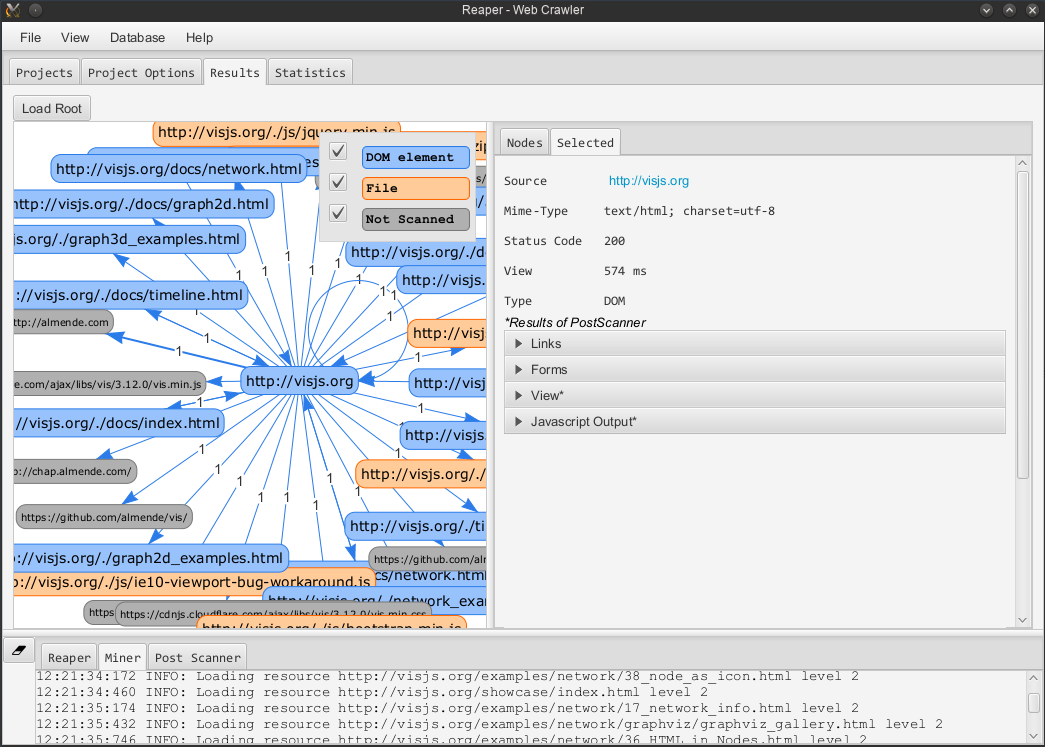
\includegraphics[scale=0.5]{reaper-results}
  \caption{V�sledky anal�zy} \label{fig:reaper_results}
\end{figure}

V~z�lo�ce statistik jsou zobrazeny dva grafy s~tabulkou jejich hodnot. Lev� graf reprezentuje z~jak�ch webov�ch objekt� v~jak�m mno�stv� je slo�ena prohledan� oblast. V~prav�m grafu je mo�no vid�t jak� odpov�di serveru byly vr�ceny. Nutno podotknout �e nap�. chybu 404 mnoh� webov� str�nky nevrac� spr�vn�, u�ivateli je zobrazeno hl�en�, �e hledan� obsah nebyl nalezen, server ale ve skute�nosti odpov� k�dem 200.

\begin{figure}[H]
  \centering
  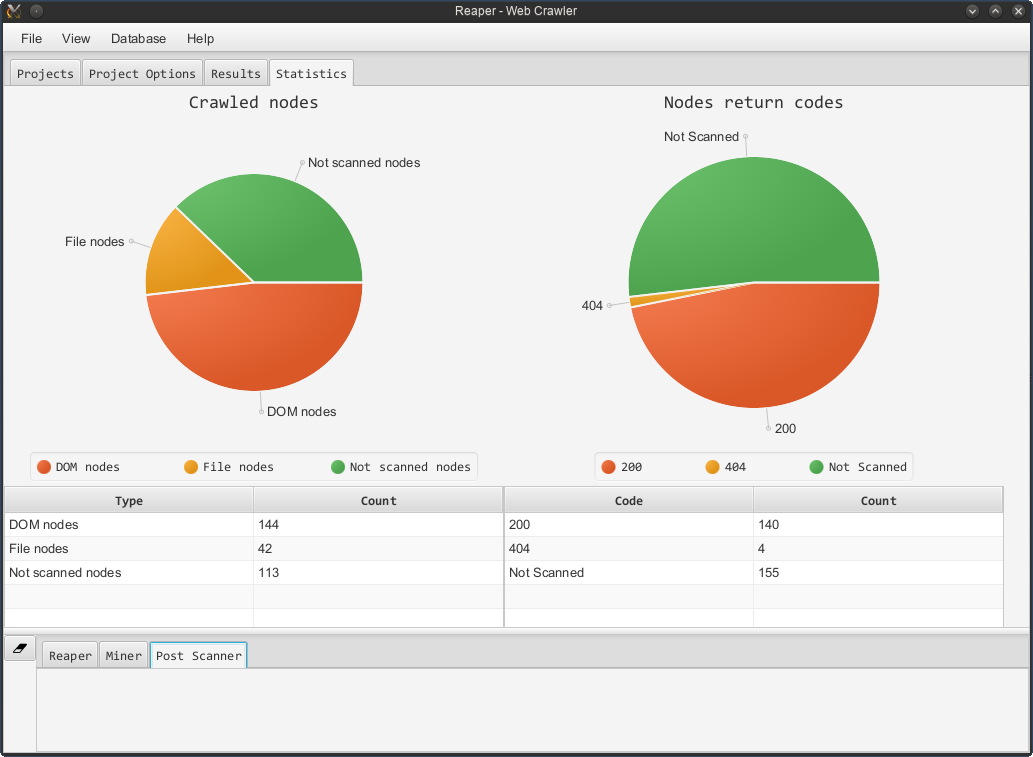
\includegraphics[scale=0.5]{reaper-stats}
  \caption{Statistiky} \label{fig:reaper_stats}
\end{figure}


\section{Webov� rozhran�}
\label{sec:web_interface}
P�vodn� pl�n t�to pr�ce bylo tak� aplikaci v~ur�it�m bod� p�en�st do webov�ho rozhran�. U�ivatele by k~aplikaci mohli p�istoupit prost�ednictv�m sv�ho prohl��e�e. Tato mo�nost bohu�el tohoto projektu ji� nen� mo�n� z~d�vodu rychle rostouc�mi po�adavky na zdroje, kter� aplikace pot�ebuje ke sv�mu b�hu.

Dal�� z~probl�mu, kter� se v~t�to oblasti objevil je rozhodnut�, spole�nosti Google stoj�c�m za prohl��e�em Google Chrome, o~ukon�en� podpory \texttt{NPAPI} pluginu. Toto rozhodnut� bylo stanoveno do konce roku 2015, po vstupu do ��innosti nebude mo�n� spustit Java kod v~prohl��e�i Google Chrome, aplikace by tak byla podporov�na pouze v~prohl��e��ch Firefox, Internet Explorer a Safari.

Mo�n� �e�en� tohoto probl�mu by byl n�vrh �ist� webov� aplikace, kter� by m�la p��stup k~vytvo�en� datab�zi a z�rove� k~souborov�mu syst�mu s~ulo�en�mi vykreslen�mi sn�mky anal�zy. Bohu�el toto �e�en� vy�aduje p��li� velk� mno�stv� �asu a zna�n� by t�m utrp�li ostatn� body t�to pr�ce.
\newpage
\chapter{V�sledky}
\label{ch:experiments}
Experimenty jsem prov�d�la na n�sleduj�c� konfiguraci.
\begin{table}[H]
  \begin{center}
    \begin{tabular}{| c | l |}
      \hline
      CPU & FX-6300 3,5GHz \\
      \hline
      RAM & 12GB DDR3 \\      
      \hline
      OS & Fedora 20 \\
      \hline
      Java & JDK 1.8.40 \\
      \hline
    \end{tabular}
  \end{center}
  \caption{HW/SW konfigurace} \label{tab:db_classes}
\end{table}

Anal�zy jsem prov�d�la na dom�n�ch s~r�zn�m po�tem webov�m objekt�. Dom�ny ozna�en� jako men�� ozna�uji ve�ker� dom�ny jejich� anal�za objevila m�n� jak 1000 objekt�. Dom�ny jako v�t�� ozna�uji v�echny ty, kter� toto ��slo p�es�hly. 

Spot�eba RAM pam�ti aplikace po n�kolika hodin�ch spu�t�n� anal�zy nep�ekro�ila 1 GiB. Toto pova�uji za velik� �sp�ch, proto�e se t�m poda�ilo vy�e�it probl�my prototypu zm�n�n� v~kapitole n�vrhu aplikace \ref{ch:plan}. Na �kor spot�eby zdroj� aplikace se projevil pot�ebn� �as k~dokon�en� anal�zy. U~dom�n skl�daj�c�ch se z~des�tky tis�c odkaz� je anal�za velice pomal�, nap�. anal�za port�lu seznam.cz se dostala do t�et� �rovn� odkazu a� po n�kolika hodin�ch. 

��dn� anal�za dom�n s~v�t��m po�tem objekt� nebyla dokon�ena b�hem jednoho spu�t�n�. St�valo se, �e b�hem anal�zy vypadlo internetov� p�ipojen�, �i do�asn� neodpov�dala datab�ze. Z~t�chto d�vodu jsem provedla �pravy v~programu aby ve�ker� data b�hem anal�zy se ukl�daly do datab�ze, v�sledkem tohoto sna�en� jsou t��dy \texttt{LinkQue} a \texttt{LinkSet}. V~p��pad� op�tovn� spu�t�n� anal�zy, aplikace pokra�uje v~anal�ze kde p�edt�m p�estala.

I~p�esto tyto velk� dom�ny se mi nepoda�ilo prozkoumat do v�t��ch hloubek, se vzr�staj�c�m po�tem z�znam� v~datab�zi se rychlost zpracov�n� dotazu ��m d�l v�c zpomalovala a po n�kolika hodin�ch zpracovan� po�et odkazu se pohyboval kolem n�kolika tis�c a po�et odkaz� ve front� se neust�le zvy�oval k~n�kolika des�tk�m tis�c.

Oproti tomu anal�za obou ��st� u~men��ch dom�n trv� t�m�� v�dy pod deset minut.

\newpage
\chapter{Dal�� mo�n� roz���en�}
\label{ch:enhacements}
N�kter� ��sti t�to aplikace jsou zpracov�ny velice jednodu�e a existuje mnoho mo�nost� jak by d�l mohly roz���it. Zde je uveden seznam v�c�, kter� jsem nestihla dot�hnout do fin�ln� podoby.

Jak prvn� tak i druh� ��st anal�zy prob�h� synchronn� v~jednom vl�kn�. Tato vlastnost nevyu��v� dostate�n� zdroje po��ta�e a anal�za je z~tohoto d�vodu velmi pomal�. Prvn�m krokem k~napraven� by bylo roz���it prvn� ��st anal�zy k~vyu�it� n�kolika vl�ken. Druh� ��st anal�zy p�i ka�d�m spu�t�n� extern�ho programu �ek� na jeho ukon�en�, spou�t�n� n�kolika proces� z�rove� by se dos�hlo lep��ch v�sledk�.
Dal�� podstatn�j� n�ro�n�j�� mo�nost by bylo rozd�len� slu�eb prov�d�j�c� anal�zu a s�� klientsk�ch program� na v�ce za��zen�ch. Tyto programy by pracovaly na jedn� dom�n� sou�asn�, jako sv�j hlavn� komunika�n� prost�edek by vyu�ily datab�zi.

Krom� chyb�j�c�ho webov�ho rozhran� je nap�. z�lo�ka statistik zm�n�n� v~sekci \ref{sec:gui} chud� na d�le�it� informace. U�ivatel se m��e prost�ednictv�m grafu dozv�d�t, �e se na dom�n� nach�z� objekty, jejich� pokus o~zp��stupn�n� zp�sobil chybu 500, ale nedov� se, kter� objekty to byly.
V~z�lo�ce statistik chyb� tak� jak�koliv anal�za rychlosti p��stupu na objekty a velikosti objekt�. U�ivatele aplikace by mohlo zaj�mat, kter� ��sti webov�ch str�nek se uk�zaly jako nejpomalej�� a podrobit tyto ��sti podrobn�j��m zkoum�n�m.

P�i vyhled�v�n� a zkoum�n� formul��� se do datab�ze ukl�d� jen velmi mal� mno�stv� dat, informace o~pol�ch formul��e zcela chyb�.

Ka�d� webov� server je n���m unik�tn�, tvo�it n�stroje, kter� se sna�� ``vyhov�t v�em'' m��e b�t n�ro�n� a� nemo�n�. Pokud by aplikace podporovala mo�nost vlo�en� u�ivatelsk�ch skript� p�i pr�ci prohl��e�e ve druh� ��sti anal�zy, byl by u�ivatel schopen dodefinovat chov�n� pavouka p�i specifick�ch p��padech.

\newpage
\chapter{Z�v�r}
\label{ch:closure}

Poda�ilo se mi vytvo�it aplikaci, kter� je schopna analyzovat dom�nou a vytvo�it jej� graf v~datab�zi spolu s~�daji o~zmapovan�ch objektech. Aplikace je postavena na frameworku JavaFX a jako �lo�i�t� vyu��v� datab�zi s~grafov�m modelem OrientDB. Aplikace je tak� schopn� v�sledky anal�zy prezentovat u�ivateli. Data jsou ulo�ena na u�ivateli p��stupn� m�sto k~dal��mu zpracov�n�/vyu�it�.

Aplikace si neklade p��li� velk� n�roky na dostupn� prost�edky. Nam�sto toho zpomaluje celkov� �as anal�zy. Z~experiment� je mo�n� vyvodit, �e aplikace nen� vhodn� na anal�zu dynamick�ch a obsahov� rozs�hl�ch dom�n. P�esto se m��e projevit u�ite�n� pro dom�ny s~men��m a hlavn� statick�m obsahem. P�i opakovan�m spu�t�n� m��eme pozorovat zm�ny v~struktu�e webov�ch objekt� i jejich mno�stv�.

Webov� prezentace dat v~aplikaci chyb�, ale v~sekci \ref{sec:web_interface} bylo navrhnuto �e�en�. P�i implementaci aplikace m� napadlo mno�stv� dal��ch roz���en� a sm�r�, kam by v�voj aplikace mohl d�le pokra�ovat, tyto roz���en� jsou pops�na v~kapitole \ref{ch:enhacements}.

%=========================================================================
 % viz. obsah.tex

  % Pouzita literatura
  % ----------------------------------------------
\ifczech
  \bibliographystyle{czechiso}
\else 
  \bibliographystyle{plain}
%  \bibliographystyle{alpha}
\fi
  \begin{flushleft}
  \bibliography{literatura} % viz. literatura.bib
  \end{flushleft}
  \appendix
  
  \chapter{Obsah CD}

\begin{itemize}
 \item Slo�ka \texttt{src}
  \begin{itemize}
   \item Zdrojov� soubory aplikace.
  \end{itemize}
 \item Slo�ka \texttt{dist}
 \begin{itemize}
  \item P�elo�en� bal��ky apletu a desktopov� verze aplikace.
 \end{itemize}
 \item Slo�ka \texttt{libs}
 \begin{itemize}
  \item Knihovny pot�ebn� k p�elo�en�.
 \end{itemize}


\end{itemize}

%\chapter{Manual}
%\chapter{Konfigra�n� soubor}
%\chapter{RelaxNG Sch�ma konfigura�n�ho soboru}
%\chapter{Plakat}

 % viz. prilohy.tex
\end{document}
